\section{Durchführung}
\label{sec:Durchführung}
Zur Durchführung des Versuchs wird der in Abbildung (\ref{fig:Versuchsaufbau}) zu sehende Versuchsaufbau
verwendet. 
\begin{figure}[H]
    \centering
    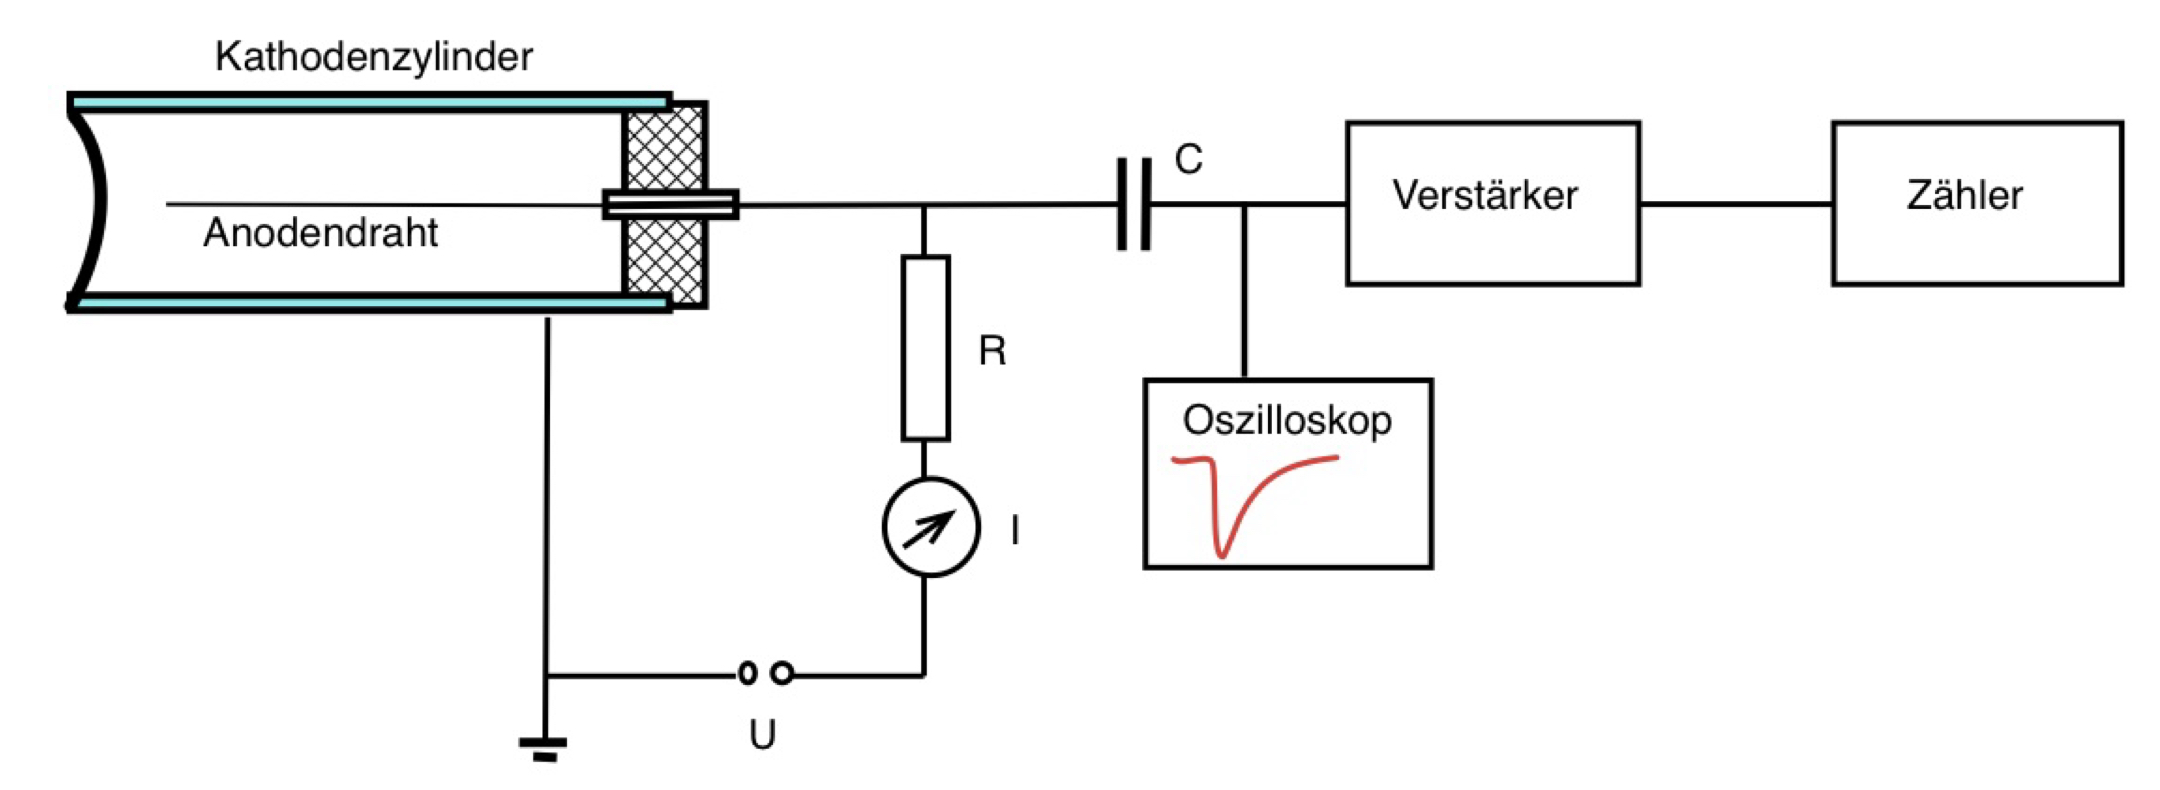
\includegraphics[width=\textwidth]{content/Bilder/Gesamte_Schaltung.jpeg}
    \caption{Schematischer Versuchsaufbau. \cite{anleitungV703}}
    \label{fig:Versuchsaufbau}
\end{figure}
\subsection{Vermessung der Kennlinie}
Zur Vermessung der Kennlinie wird die radioaktive Quelle 
vor den Detektor gestellt und die Zählrate über einen 
Zeitraum von $\Delta t = 60 \, \unit{\second}$ bei variierender
Spannung gemessen. Als Anfangsspannung wird $300 \, \unit{\volt}$
eingestellt. Die Spannung wird danach in Schritten von $20 \, \unit{\volt}$
erhöht bis bei $780 \, \unit{\volt}$ ein sprunghafter Anstieg der
Zählrate zu vermerken ist. Dies markiert den Übergang vom Geiger-Müller-Bereich 
in den Dauerentladungsbereich. 
\subsection{Bestimmung der Totzeit}
Zur Bestimmung der Totzeit werden zwei Methoden angewendet. Die erste Methode besteht 
darin auf dem Oszilloskop die Totzeit abzulesen. 
Die zweite Methode ist die Zwei-Quellen-Methode. Dazu wird eine bestimmte Spannung als
Arbeitspunkt gewählt, die im ersten drittel des Geiger-Müller-Plateaus liegt. Anschließend
wird die Zählrate der beiden verschiedene Quellen und die Zählrate beider Quellen 
zusammen vermessen. Jede Zählrate wird über ein Zeitintervall von 
$\Delta t = 120 \, \unit{\second}$ gemessen. 